% $Header: /cvsroot/latex-beamer/latex-beamer/solutions/generic-talks/generic-ornate-15min-45min.en.tex,v 1.5 2007/01/28 20:48:23 tantau Exp $

\documentclass{beamer}

% This file is a solution template for:

% - Giving a talk on some subject.
% - The talk is between 15min and 45min long.
% - Style is ornate.



% Copyright 2004 by Till Tantau <tantau@users.sourceforge.net>.
%
% In principle, this file can be redistributed and/or modified under
% the terms of the GNU Public License, version 2.
%
% However, this file is supposed to be a template to be modified
% for your own needs. For this reason, if you use this file as a
% template and not specifically distribute it as part of a another
% package/program, I grant the extra permission to freely copy and
% modify this file as you see fit and even to delete this copyright
% notice. 


\mode<presentation>
{
  \usetheme{Warsaw}
  % or ...

  \setbeamercovered{transparent}
  % or whatever (possibly just delete it)
}


\usepackage[spanish]{babel}
% or whatever

\usepackage[utf8]{inputenc}
% or whatever

\usepackage{times}
\usepackage[T1]{fontenc}
% Or whatever. Note that the encoding and the font should match. If T1
% does not look nice, try deleting the line with the fontenc.
\usepackage{hyperref}

\title{Software libre en la escuela}

\author{Germán Avendaño Ramírez~\thanks{Lic. Mat. U.D.; M.Sc. U.N.}}
% - Use the \inst{?} command only if the authors have different
%   affiliation.

\institute[Universities of Somewhere and Elsewhere] % (optional, but mostly needed)
{
  \inst{}%
  Docente de Matemáticas\\
  Colegio Arborizadora Baja I.E.D.\\
  \vskip5mm
  Delegado a la Asamblea\\
  ADE
  }
% - Use the \inst command only if there are several affiliations.
% - Keep it simple, no one is interested in your street address.

\date{Septiembre 23 de 2016}

\subject{Talks}
% This is only inserted into the PDF information catalog. Can be left
% out. 



% If you have a file called "university-logo-filename.xxx", where xxx
% is a graphic format that can be processed by latex or pdflatex,
% resp., then you can add a logo as follows:

% \pgfdeclareimage[height=0.5cm]{university-logo}{university-logo-filename}
% \logo{\pgfuseimage{university-logo}}



% Delete this, if you do not want the table of contents to pop up at
% the beginning of each subsection:

% If you wish to uncover everything in a step-wise fashion, uncomment
% the following command: 

%\beamerdefaultoverlayspecification{<+->}


\begin{document}

\begin{frame}
  \titlepage
\end{frame}

\begin{frame}{Para reflexionar y debatir}
  \tableofcontents
  % You might wish to add the option [pausesections]
\end{frame}


% Since this a solution template for a generic talk, very little can
% be said about how it should be structured. However, the talk length
% of between 15min and 45min and the theme suggest that you stick to
% the following rules:  

% - Exactly two or three sections (other than the summary).
% - At *most* three subsections per section.
% - Talk about 30s to 2min per frame. So there should be between about
%   15 and 30 frames, all told.

\section{Resumen}
\begin{frame}{Resumen}
En esta breve ponencia se tratará de definir que es el software libre y por qué debe usarse solamente éste en la escuela
\end{frame}
\section[Introducción]{Introducción}
\begin{frame}{Introducción}
En la escuela se deben formar estudiantes autónomos, críticos y capaces de transformar la realidad. Para asegurar que nuestros estudiantes sean autónomos de verdad, no se les debe enseñar en la escuela a depender de software privativo para desarrollar sus tareas académicas, habiendo tanto software alternativo y libre. Si se enseña software privativo estaremos creando seres dependientes de las grandes multinacionales que manejan el software privativo como Microsoft, Apple, etc.
\end{frame} 
\section{¿Qué es el software libre?}
\begin{frame}
\begin{center}
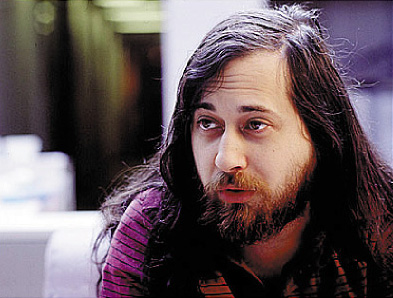
\includegraphics[scale=.5]{Richard_Matthew_Stallman.jpeg} 
\end{center}
El software libre fue definido por Richard Mathew Stallman en la década de 1980. Éste debe respetar las 4 libertades esenciales \cite{gnu}
\end{frame} 
\begin{frame}{Las cuatro libertades esenciales}
\begin{itemize}
  \item La libertad de ejecutar el programa, para cualquier propósito. \alert{Libertad 0}
  \pause
  \item La libertad de estudiar cómo trabaja el programa, y cambiarlo para que haga lo que usted quiera. El acceso al código fuente es una condición necesaria para ello. \alert{Libertad 1}
  \pause
  \item La libertad de redistribuir copias para que pueda ayudar al prójimo. \alert{Libertad 2}
  \pause
  \item La libertad de distribuir copias de sus versiones modificadas a terceros. Si lo hace, puede dar a toda la comunidad una oportunidad de beneficiarse de sus cambios. El acceso al código fuente es una condición necesaria para ello. \alert{Libertad 3}
  \end{itemize}
\end{frame}
\begin{frame}{El mismo RMS hablando}
Ver vídeo de Richard Stallman sobre "Software libre y educación" (6 minutos de duración)\\
\url{www.gnu.org/education/rms-education-es.ogv}\cite{rms}
\end{frame}
\subsection{¿Cuál es la relación entre el software libre y la educación?}
\begin{frame}{Sociedad, Ética y política}
La educación debe formar en y para la libertad. Además de la libertad, en la escuela se deben formar individuos que sirvan a su comunidad. El software privativo es conocimiento secreto y restringido, por lo tanto se opone a las misiones de las instituciones educativas. El software libre por el contrario educa en la libertad y la cooperación.

El software libre no es simplemente un asunto meramente técnico sino que adquiere connotaciones éticas sociales y políticas. Es una cuestión de derechos humanos que los usuarios deben tener.\cite{rms}
\end{frame}
\subsection{Por qué las escuelas solamente deben enseñar software libre}
\begin{frame}{¿Por qué tanta preocupación?}
Hay muchas razones por las cuales en las escuelas solamente debemos enseñar software libre. Entre algunas tenemos:\cite{esc}
\end{frame}
\begin{frame}{Razones para elegir solamente software libre en nuestras escuelas}
\begin{itemize}  
\item El software libre le brinda al usuario la libertad de saber que hacen realmente los programas instalados en sus dispositivos.Se sabe que muchos programas del software privativo tienen las denominadas puertas traseras (backdoors) que permiten a los gobiernos y/o multinacionales espiar a sus usuarios\footnote{Es famoso el caso de Amazon con su dispositivo Kindle. A miles de usuarios que habían obtenido el libro 1984 de H.G. Wells gratuitamente, les fue borrado remotamente porque su contenido no les pareció ``apto''}
\end{itemize}
\end{frame}
\begin{frame}{\ldots Continúan las razones}
\begin{itemize}
\item Supone un ahorro económico porque no se deben pagar onerosas licencias. El software libre generalmente es muy económico y en la mayoría de los casos es gratuito.\pause
\item Permite saber a los y las estudiantes como funciona el software y así desarrollar habilidades para que no seamos solamente un país consumidor de tecnología, sino que seamos capaces de crear nuestros propios programas.\pause
\item La razón más profunda tiene que ver con la \alert{educación moral}. Se espera que en la escuela se enseñe a nuestros estudiantes a ser buenos ciudadanos lo cual implica enseñarles el hábito de ayudar a los demás.
\end{itemize}
\end{frame}
\begin{frame}{\ldots Y siguen las razones}
\begin{itemize}
\item Enseñar software privativo es crear dependencia de las multinacionales, que se reservan el derecho de esconder el código fuente (\alert{código ofuscado}) para que no sepamos realmente que hacen los programas, éstos pueden hacer cosas adicionales que no queremos que hagan, como por ejemplo espiarnos. Las grandes empresas del software quieren crear seres dependientes de su software, por eso a veces hasta regalan copias de sus programas para crear dependencia como hacen los expendedores de drogas, que regalan la primera dosis a sus futuros compradores. Luego de que egresen nuestros estudiantes no sabrán operar sino software privativo y luego allí si tendrán que pagar las licencias. 
\end{itemize}
\end{frame}
\section{Software libre útil en la escuela}
\begin{frame}{Alternativas la software privativo}
\begin{center}
\textbf{Alternativas al software privativo}
\begin{tabular}{|l|l|}
\hline 
\textbf{Aplicación libre} & \textbf{Aplicación privativa }\\ 
\hline 
Libreoffice & Microsoft office \\ 
\hline 
Gimp & Adobe PhotoShop \\ 
\hline 
Inkscape & Adobe illustrator \\  
\hline 
mplayer, smplayer, vlc & Reproductor de Windows M \\ 
\hline 
Audacious, amarok, clementine & Winamp \\ 
\hline 
Firefox, midori, chromium \ldots & Chrome, Internet Explorer \ldots\\ 
\hline 
\end{tabular} 
\end{center}
\end{frame}
\begin{frame}
Para la educación tenemos un abanico de posibilidades. Para cada una de las áreas de la educación y cada una de nuestras necesidades tenemos a nuestra disposición suficientes aplicaciones que podemos usar con la tranquilidad de que no estamos haciendo algo ilegal, ya que éstas hacen uso de las licencias del software libre (GPL, GPL2, etc). A continuación una tabla con las aplicaciones alternativas al software privativo más usual.
\end{frame}
\begin{frame}{Software libre para educar}
\begin{tabbing}
\hspace{4cm}\=\kill
Matemáticas \> Geogebra, kig, drgeo, kbruch, kalgebra, etc \\ 
Geografía \> kgeography, marble, etc \\ 
Idiomas \> Goldendict, kletters, khangman, etc \\ 
Química \> chemtool, easychem, gperiodic, kalzium\\
Música \> Denemo, solfege,etc \\ 
\ldots \> \ldots
\end{tabbing} 
\end{frame}

\section{Conclusiones}
\begin{frame}{¿Qué debemos hacer?}
Es urgente dar un viraje en cuanto al uso de las TICS en nuestras escuelas, porque el movimiento que impulsa éstas, no se ha detenido a mirar que podemos estar cayendo en el uso de aplicaciones que no permitirán a los futuros ciudadanos ser libres, sino que generaremos dependencia. Es necesario analizar las implicaciones éticas, sociales y políticas de continuar usando en nuestras aulas software privativo.
\end{frame}
\section*{Bibliografía}
\begin{frame}[allowframebreaks]
  \frametitle<presentation>{Lecturas recomendadas}
    
  \begin{thebibliography}{10}
    
%  \beamertemplatebookbibitems
  % Start with overview books.
  
  \beamertemplatearticlebibitems
  % Followed by interesting articles. Keep the list short. 

\bibitem{gnu} \emph{Stallman Richard, Proyecto GNU}
 \newblock{¿Que es el software libre?}
 \newblock {\url{www.gnu.org/philosophy/free-sw.es.html}}

  \bibitem{rms} \emph{Stallman Richard}
  \newblock{¿Cuál es la relación entre software libre y la educación?} \newblock{\url{www.gnu.org/education/education.es.html}}
  
\bibitem{esc} \emph{Stallman Ricard}
\newblock{Por qué las escuelas deben enseñar únicamente software libre}  \newblock{\url{www.gnu.org/education/edu-schools.es.html}}
  \end{thebibliography}
\end{frame}

\end{document}
